\chapter{Implementation And Testing}

	\section{The actual implementation of the software}
	%%TODO pensare se c'è da aggiungere qualcosa

	The image \ref{} shows the class diagram of the implementation of the software. 
	According to the design specifications defined in chapter \ref{chDesign}, the software is organized in four main parts, each of them has its own role.
	Both the feature extractor and the class hierarchy components are made up by the same classes defined in chapter \ref{chDesign}. 
	The parts containing the utility functions and the features for the communication with \mbox{ACT-R} have been extended and completed in order to reach the goal for which they have been introduced.
	The following sections describe the implementation for this two latter parts.
	
	\subsection{Utility Part}
	The utility part is composed by the classes \emph{InputException},\emph{NotOverlappedSegmentException},\emph{ParallelLinesException},\emph{VerticalLineException},\emph{CoincidentLinesException}, \emph{FourPointsSorter}, \emph{StraightLine},\emph{Segment}, \emph{Point}, and another module containing functions. The latter, as it is not a class, is not included in the diagram in figure \ref{}. 

	\emph{InputException},\emph{NotOverlappedSegmentException},\emph{ParallelLinesException},\emph{VerticalLineException},\emph{CoincidentLinesException} are exceptions classes, used to handle all the anomalous or exceptional events occurring during the execution of the software. 

	\emph{StraightLine},\emph{Segment} and \emph{Point} represent geometrical entities. Such elements are fundamental structures for creating the objects in the hierarchy and making evaluations, both qualitative and quantitative, between couples of objects, as, for example, the distances between two centers or the relative positions.

	\emph{FourPointsSorter} and the module containing contain the basic methods which are fundamental for all the operations executed by all the other classes of the software.

	The part responsible for the communication with the cognitive architecture is composed by the classes \emph{Server} and \emph{Session}. 
	


 
	\section{Testing}
\begin{comment}

	As it can be seen in the picture, the software is logically divided in the four main components introduced in the design chapter (see \ref{chDesign}).
%, respecting the in the design specifics described in chapter \ref{chDesign}. 
	Both the feature extraction part and the class hierarchy respect the design specifications, described in such chapter. The classes responsible for the communication with \mbox{ACT-R} and the utility part.
The communication with  and


	\newpage
	
	\begin{sidewaysfigure}[hbtp]
	   \thispagestyle{empty}	
 	   \centering
	   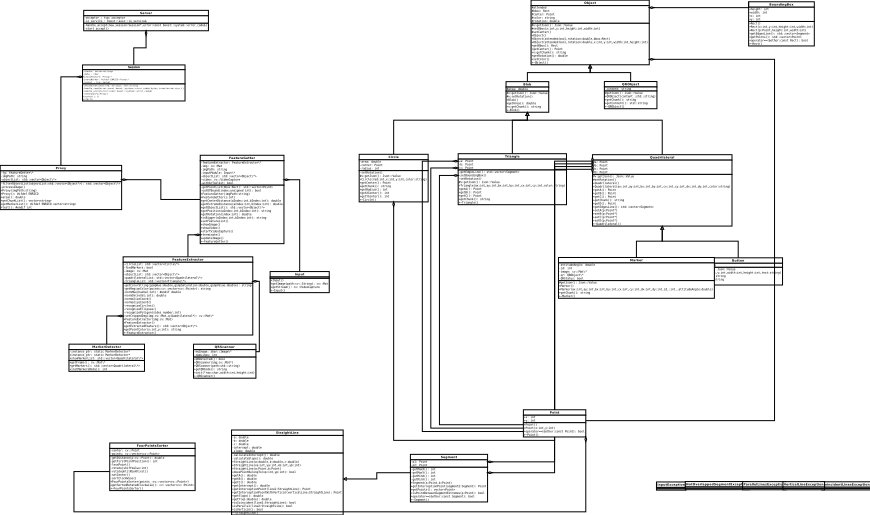
\includegraphics[height=\textheight]{images/ch_06/implementation.jpg}
	   
	  \caption{\textit{Class diagram illustrating the class hierarchy of the recognized objects}}  
	  \label{fig:HierarchyDesign}
 	\end{sidewaysfigure}

\newpage

\relax
	\AddToShipoutPicture*{ \\ \relax
	  \setlength{\unitlength}{1mm} 
	  \put(<10>, <10>){  
	    \makebox(0,0){\includegraphics{images/ch_05/feature.png}}}} 
	ciao

	
\end{comment}

	\section{COmmunication with ACT-R}
	ciao
